\section{Auswertung}
\label{sec:auswertung}

Im Folgenden erfolgt die Auswertung der verschiedenen Messungen.

\subsection{Bestimmung der freien Weglänge}

Zunächst soll mit den Erkenntnissen aus \autoref{sec:einflüsse:dampfdruck}
die mittlere freie Weglänge $\bar{w}$ der Elektronen im \ce{Hg}-Dampf bestimmt werden.

% laut Versuchsanleitung:
Diese ist in $\si{\centi\meter}$ gegeben durch
\begin{equation*}
    \bar{w} = \frac{\num{0.0029}}{p_\text{sät}}
\end{equation*}
mit
\begin{equation*}
    p_\text{sät} = \num{5.5e7} \exp{\left(\frac{-6876}{T}\right)} \ ,
\end{equation*}
wobei $T$ in $\si{\kelvin}$ gegeben sein muss
und $p$ in $\si{\milli\bar}$ resultiert.

Für die im Folgenden auftretenden Temperaturen wurden die entsprechenden Werte berechnet
und in \autoref{tab:freie_weglaenge} aufgelistet.
Dort ist auch $\sfrac{a}{\bar{w}}$ angegeben;
dieses Verhältnis von Beschleunigungsstrecke $a \approx \SI{1}{\centi\meter}$ % laut Versuchsanleitung
zu freier Weglänge $\bar{w}$
soll etwa 1000 bis 4000 betragen,
damit eine ausreichende Stoßwahrscheinlichkeit gegeben ist.
Mit Ausnahme des Werts zu Zimmertemperatur trifft dies zu.

\begin{table}
  \centering
  \caption{Freie Weglänge und weitere Größen in Abhängigkeit der Temperatur.}
  \label{tab:freie_weglaenge}
  \begin{tabular}{S[table-format=3.1] S[table-format=3.1] S[table-format=2.5] S[table-format=2.6] S[table-format=4.2]}
  \toprule
  {$T \mathbin{/} \si{\celsius}$} &
  {$T \mathbin{/} \si{\kelvin}$} &
  {$p_\text{sät} \mathbin{/} \si{\milli\bar}$} &
  {$\bar{w} \mathbin{/} \si{\milli\meter}$} &
  {$\sfrac{a}{\bar{w}}$} \\
  \midrule
  \expandableinput{build/tab/freie_weglaenge.tex}
  \bottomrule
  \end{tabular}
\end{table}


\subsection{Energieverteilung der beschleunigten Elektronen}
\label{sec:auswertung:energieverteilung}

Zunächst mussten die mit dem XY-Schreiber aufgenommenen Messwerte digitalisiert
und die Skaleneinheiten umgerechnet werden.
Die Digitalisierung erfolgte mithilfe des \href{https://automeris.io/WebPlotDigitizer/}{WebPlotDigitizer}.
Dabei wurde die vorgedruckte Skala verwendet.
Neben den Messwerten wurden aber auch die im Abstand von $\SI{1}{\volt}$ gesetzen Skalenpunkte digitalisiert,
um deren durchschnittliche Breite und Verschiebung relativ zur vorgedruckten Skala zu bestimmen.
Mithilfe dieser Informationen können schließlich die Messwerte in SI-Einheiten angegeben werden.
% Sie finden sich in \autoref{tab:mess_energieverteilung}.
% Auf eine tabellarische Auflistung dieser Messwerte wird an dieser Stelle aus Platzgründen verzichtet.
Auf eine tabellarische Auflistung der verwendeten Messwerte wird an dieser Stelle verzichtet,
weil sie ohnehin in nahezu beliebiger Anzahl
aus den mit dem XY-Schreiber gezeichneten Graphen
(siehe \autoref{fig:mess_energieverteilung})
entnommen werden können.


\autoref{fig:energieverteilung_int} zeigt nun die digitalisierten Messwerte:
In zwei Graphen ist der Auffängerstrom $I_\text{A}$ in Abhängigkeit von der Bremsspannung $U_\text{A}$
für die jeweilige Temperatur aufgetragen.

Es sei erwähnt, dass hier und in den folgenden Plots die Skala für $I_\text{A}$ fehlt,
weil Absolutwerte hierzu weder genau bekannt sind,
noch für die Auswertung benötigt werden.

\begin{figure}[H]
    \centering
    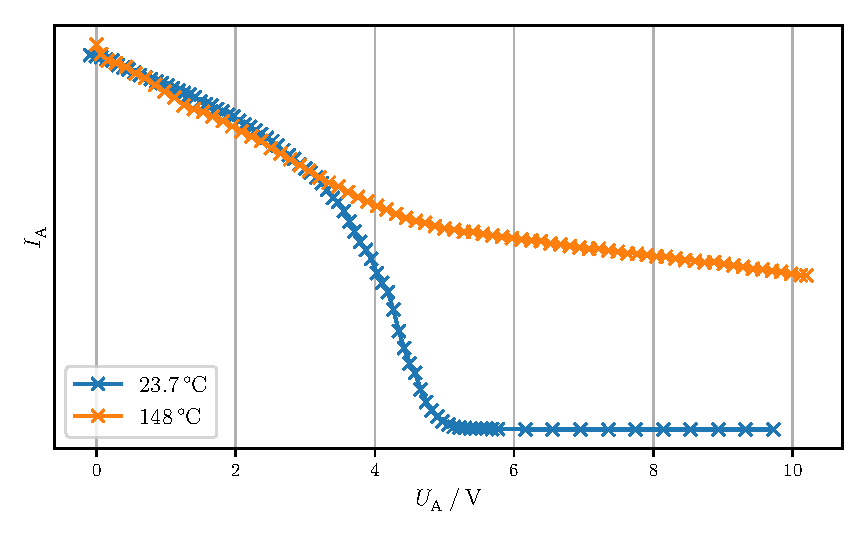
\includegraphics[width=\textwidth]{build/plt/energieverteilung_int.pdf}
    \caption{Messwerte zur integralen Energieverteilung der beschleunigten Elektronen.}
    \label{fig:energieverteilung_int}
\end{figure}


Um die differenzielle Energieverteilung zu erhalten,
werden stückweise Differenzenquotienten gemäß
\[ f\left( \frac{x_i + x_{i+1}}{2} \right) = \frac{y_{i+1} - y_i}{x_{i+1} - x_i} \]
berechnet,
wobei $x$ und $y$ hier für $U_\text{A}$ bzw. $I$ stehen.
Die daraus resultierenden Graphen sind in \autoref{fig:energieverteilung_diff} abgebildet.
%
%% Wenn ich die Messwerte gar nicht angebe, ist das auch egal… ↓
% Um aussagekräftige Ergebnisse zu erzielen,
% wurde nur jeder dritte Messwert der integralen Energieverteilung betrachtet.

\begin{figure}[H]
    \centering
    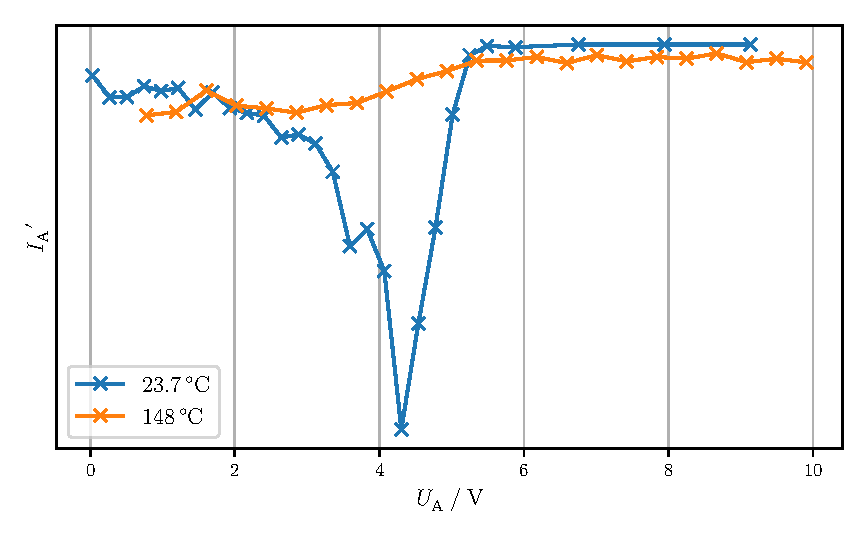
\includegraphics[width=\textwidth]{build/plt/energieverteilung_diff.pdf}
    \caption{Aus der integralen Energieverteilung berechnete Werte zur differenziellen Energieverteilung der beschleunigten Elektronen.}
    \label{fig:energieverteilung_diff}
\end{figure}

% TODO: Mist-Wert für die hohe Temperatur!?
Die Minima der differenziellen Energieverteilung liegen bei
$\SI{4.304}{\volt}$ für $T = \SI{23.7}{\celsius}$
beziehungsweise $\SI{0.142}{\volt}$ für $T = \SI{148}{\celsius}$.

Die meisten Elektronen haben also eine Energie von
$\SI{4.304}{\electronvolt}$ beziehungsweise $\SI{2.851}{\electronvolt}$.

% Auffällig ist die nicht verschwindende Breite des Peaks, auf welche in der Diskussion eingegangen wird.
% → Fermi-Dirac

Das Kontaktpotential lässt sich durch Umstellen von \autoref{eqn:kontaktpotential_verschiebung} bestimmen:
\begin{align*}
  U_\text{B,eff} &= U_\text{B} - K \\
  \Leftrightarrow
  K &= U_\text{B} - U_\text{B,eff} \ .
\end{align*}

Es folgt:
\begin{align*}
  K &= \SI{11}{\volt} - \SI{4.304}{\volt} = \SI{6.696}{\volt}
  \tag{$T = \SI{23.7}{\celsius}$} \\
  K &= \SI{11}{\volt} - \SI{2.851}{\volt} = \SI{8.149}{\volt}
  \tag{$T = \SI{148}{\celsius}$} \ .
\end{align*}


\clearpage
\subsection{Anregungsenergie des \texorpdfstring{\ce{Hg}}{Hg}-Atoms}

\autoref{fig:franck_hertz_kurve_1} und \autoref{fig:franck_hertz_kurve_2}
zeigen die für unterschiedliche Temperaturen gemessenen Franck-Hertz-Kurven.
Die Messwerte wurden aus \autoref{fig:mess_franck_hertz} entnommen.

\begin{figure}
    \centering
    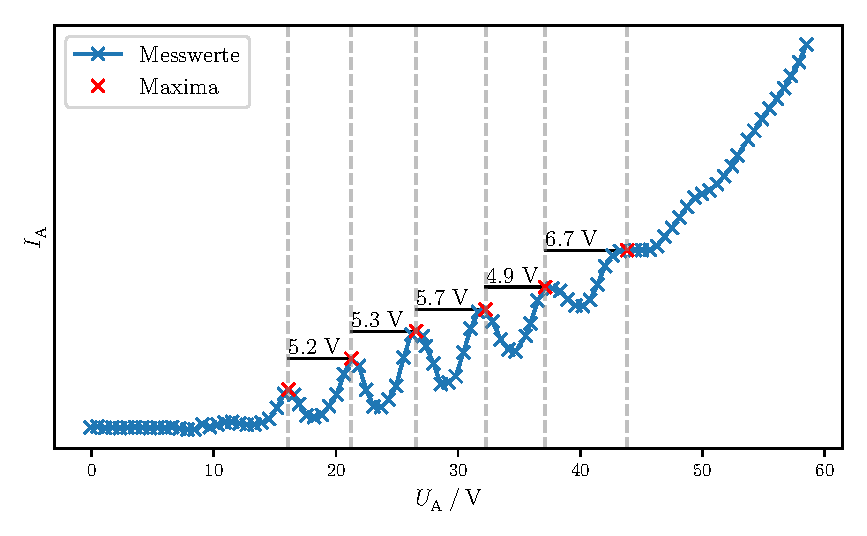
\includegraphics[width=\textwidth]{build/plt/franck_hertz_166_6.pdf}
    \caption{Franck-Hertz-Kurve für $T = \SI{166.6}{\celsius}$.}
    \label{fig:franck_hertz_kurve_1}
\end{figure}

\begin{figure}
    \centering
    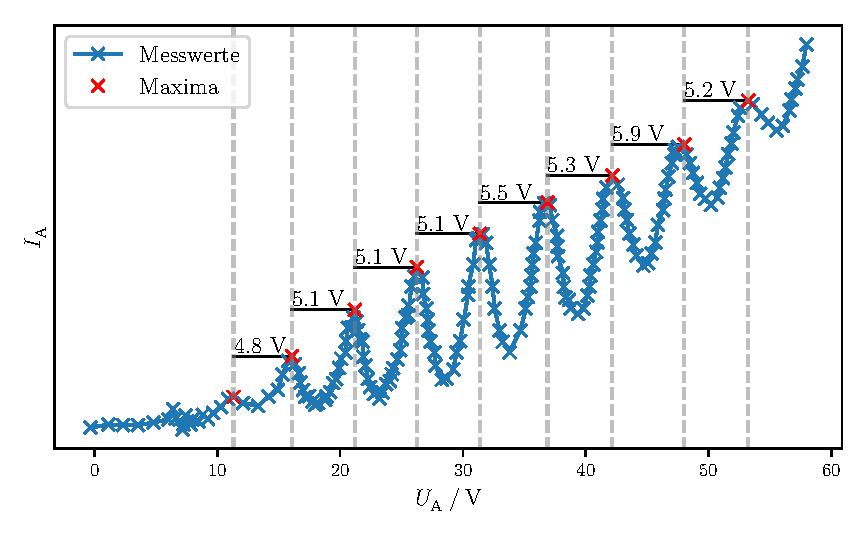
\includegraphics[width=\textwidth]{build/plt/franck_hertz_183_8.pdf}
    \caption{Franck-Hertz-Kurve für $T = \SI{183.8}{\celsius}$.}
    \label{fig:franck_hertz_kurve_2}
\end{figure}

Weil die \hyperref[fig:franck_hertz_kurve_2]{Franck-Hertz-Kurve für $T = \SI{183.8}{\celsius}$}
mehr und deutlichere Peaks aufweist,
ist diese zur Auswertung besser geeignet.
Im den folgenden Erläuterungen wird diese daher exklusiv betrachtet.
Der Vollständigkeit halber sind in \autoref{tab:franck_hertz_auswertung}
aber auch die Werte zur anderen Franck-Hertz-Kurve angegeben.


Das erste gut sichtbare Maximum des Auffängerstroms liegt bei $U_{B,0} = \SI{11.318}{\volt}$.
Mit dem mittleren Abstand der Peaks zueinander $\overline{\symup{\Delta}U_\text{B}} = \SI{5.24(12)}{\volt}$
ergibt sich somit aus \autoref{eqn:kontaktpotential_verschiebung}
ein Kontaktpotential von $K = U_{B,0} - \overline{\symup{\Delta}U_\text{B}} = \SI{6.08(12)}{\volt}$.

Aus dem Zusammenhang
\[
  E = \frac{hc}{\lambda} \Leftrightarrow
  \lambda = \frac{hc}{E}
\]
lässt sich die Wellenlänge des emittierten Photons
zu $\lambda = \SI{237(5)}{\nano\meter}$ bestimmen.
Es handelt sich also um ultraviolette Strahlung.


\begin{table}
  \centering
  \caption{Auswertungsergebnisse zur Franck-Hertz-Kurve für verschiedene Temperaturen.}
  \label{tab:franck_hertz_auswertung}
  \begin{tabular}{c | S S}
  \toprule
  {$T \mathbin{/} \si{\celsius}$} &
  166.6 & 183.8 \\
  \midrule
  $\lambda \mathbin{/} \si{\nano\meter}$ & 223(13) & 237(5) \\
  $U_{B,0} \mathbin{/} \si{\volt}$ & 16.114 & 11.318 \\
  $\overline{\symup{\Delta}U_\text{B}} \mathbin{/} \si{\volt}$ & 5.55(32) & 5.24(12) \\
  $K \mathbin{/} \si{\volt}$ & 10.57(32) & 6.08(12) \\
  \bottomrule
  \end{tabular}
\end{table}
